%\wfigure[Figures-quill/compare-bw.pdf,\figtitle{\Muse{} bandwidth} These graphs show aggregate bandwidth for various request sizes and access types.  Quill improves bandwidth by up to 7\x{}.,fig:bandwidth]

\section{Results: \DAChell{}}
\label{sec:results-quill}

This section evaluates \DAChell{}'s performance using a collection of
microbenchmarks and database workloads.  We begin by measuring \DAChell{}'s
latency and bandwidth relative to the conventional OS-based interface.  For all
the experiments in this section, we use 8~GB of DDR3-1600 DRAM to emulate 
NVMM.  We run PMFS to provide file system access to the NVMM.

\subsection{Latency}

\DAChell{} adds overhead to each file access because its userspace library
implements POSIX compatibility and must distinguish between 
accesses that \DAChell{} should perfom and accesses should it forward to the OS.
This latency replaces some of the file
system and operating system latency that normal system calls incur.

Figure~\ref{fig:quill-latency} shows the latency of \DAChell{} for different
request sizes comparing to PMFS.  All the pages \DAChell{} and PMFS accessed
are loaded into memory before measurement begins to ensure that they are in the page table to eliminate the
\texttt{mmap()} and page fault handling overhead.
The total latency for a 4~kB read operation through \DAChell{} is 0.39~\us{} on
average, compared to 0.48~\us{} for an access to PMFS via the kernel.  For a 4~kB write,
\DAChell{} takes 0.51~\us{}, and PMFS takes 0.63~\us{}. \DAChell{} reduces 4~kB
access latency by 19\% over PMFS.  For requests smaller than 4~kB,
\DAChell{}'s performance relative to PMFS improves, because writes to the file system
involve metadata changes.

In some cases, \DAChell{} reduces performance.  In particular file operations that
modify file system metadata are slower, since \DAChell{} incurs its own overhead \emph{and} must make a system call.
Appends are the most common example.
Under \DAChell{}, a 4~kB append
takes 1.3~\us{}. Under the conventional interface, it requires just
1.1~\us{}.

Figure~\ref{fig:latency-mmap} measures the overhead of \texttt{mmap()} and page fault handling and quantifies the trade-offs between pre-loading the page tables with MAP\_POPULATE and loading pages on demand.
It shows the latency breakdown of for the first access to a page with \DAChell{}.
In the test we use \DAChell{} to read a 2~MB file
with a sequence of 4~kB requests.
Since \DAChell{} \texttt{mmap()s} 2~MB at a time,
there is only one \texttt{mmap()} call
for the file.  The graph shows the amortized cost for accessing a single page, the total \texttt{mmap()} latency is 512 times larger.
With MAP\_POPULATE disabled, \texttt{mmap()} does not populate the pages
to the page table, and the  amortized \texttt{mmap()} latency is low: only 2.6~ns
for each 4~kB access.  With MAP\_POPULATE enabled,
the amortized cost of \texttt{mmap()} is 88~ns for each page.
However, the access latency
for each page with MAP\_POPULATE enabled is 310~ns versus 612~ns
with MAP\_POPULATE disabled.  This means servicing the page miss takes 302~ns.  These data suggest that using MAP\_POPULATE is important to achieving good performance, \emph{if most pages will eventually be accessed}.
Based on the values we measured for our system, if at least 28\% pages of the 2~MB chunk will be accessed, then enabling MAP\_POPULATE improves performance.

\cfigure[Graphs/quill-latency.pdf,{\figtitle{\DAChell{} latency for different request sizes compared to PMFS with pages loaded on demand.  The cost of mmap() is amortized across the 512 pages in the 2~MB file.
}},fig:quill-latency]

\cfigure[Graphs/latency-mmap.pdf,{\figtitle{\DAChell{} 2~MB file read latency breakdown for each 4~kB access, with the MAP\_POPULATE flag set. The cost of mmap() is amortized across the 512 pages in the 2~MB file.}},fig:latency-mmap]

\ignore{
\begin{figure}
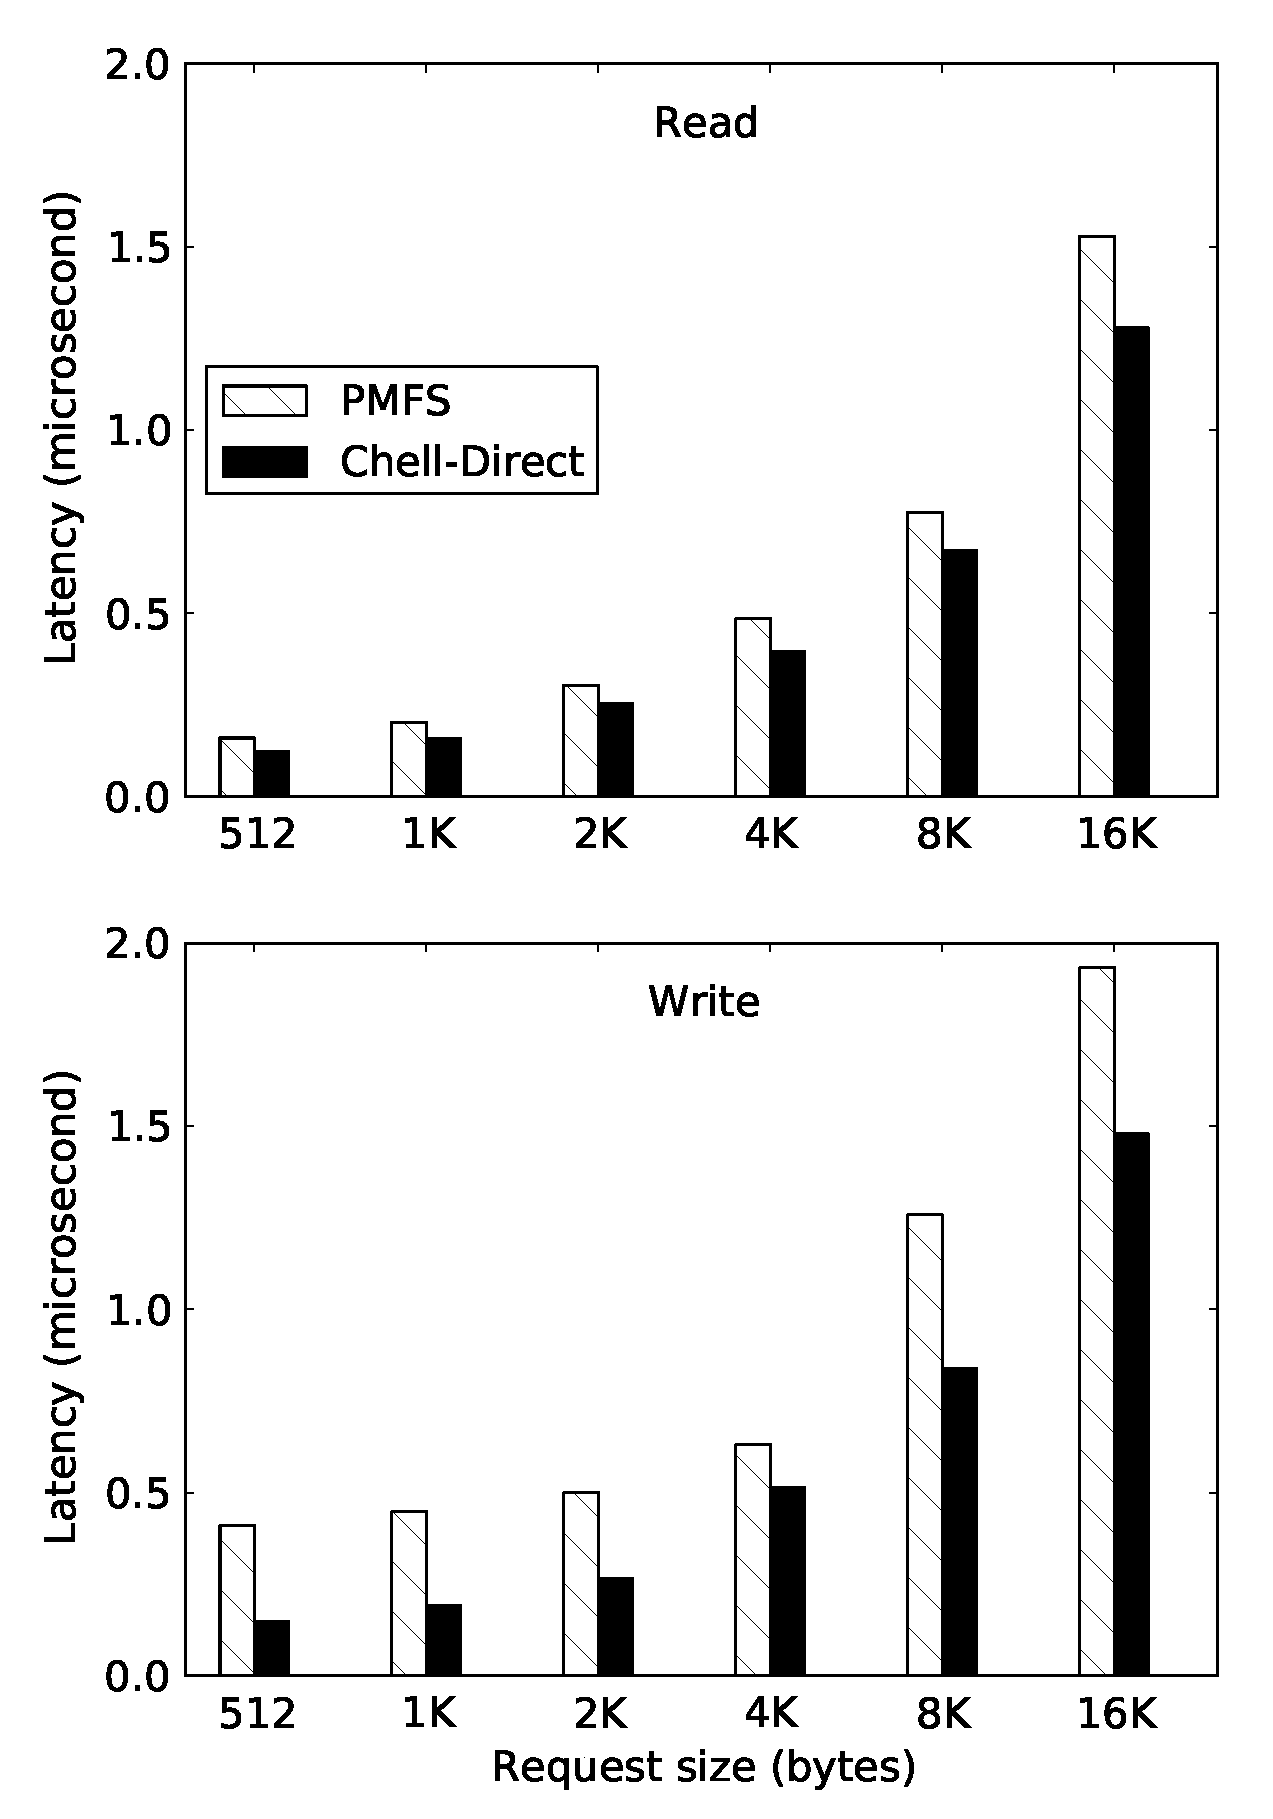
\includegraphics[width=\linewidth]{Graphs/quill-latency.pdf}
\caption{\DAChell{} latency}
\label{fig:quill-latency}
\end{figure}
}

\begin{figure*}
\vspace*{0mm}
 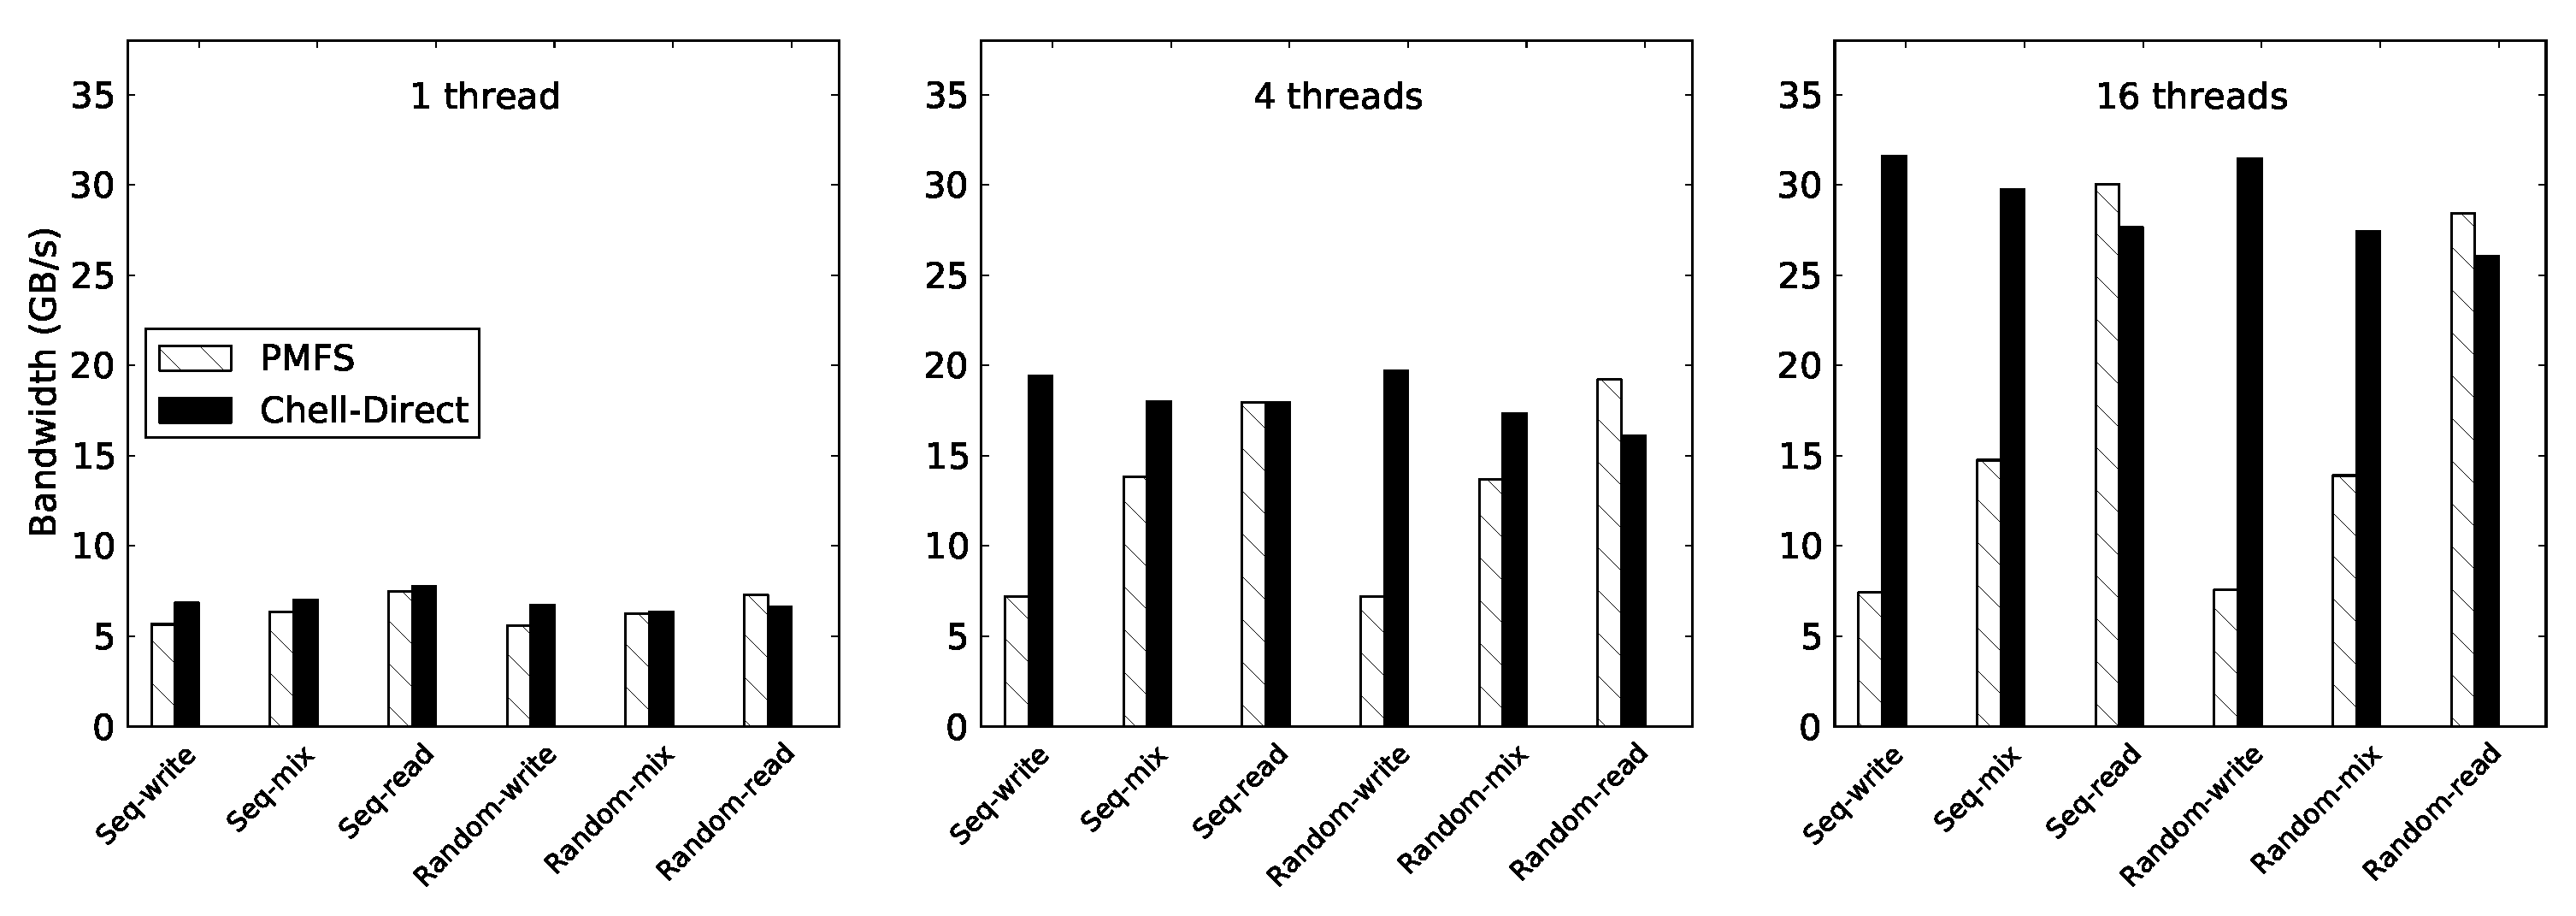
\includegraphics[width=\textwidth]{Graphs/xdd-quill.pdf}
 \vspace*{-5mm}\caption{\DAChell{} xdd bandwidth}
 \label{fig:quill-bandwidth}
\end{figure*}

\ignore{
\DAChell{} performs 
significant file read ahead.  When \DAChell{} \texttt{mmap()}s a file it creates
a memory mapping twice the size of the file.  If the file size grows, \DAChell{}
does not need to update the mapping; it just needs to increase the file size.  
If the file eventually exceeds the mapping size, \DAChell{} doubles the size of 
the mapped region.  As a result, some appends incur larger overheads, but, on
average, the overhead is small.}

\subsection{Bandwidth}

Placing storage on the processor's memory bus should provide high
bandwidth access to data.  We use Xdd~\cite{xdd} to measure bandwidth of \DAChell{}.
Figure~\ref{fig:quill-bandwidth} quantifies the bandwidth available from our
NVMM device
via PMFS and via \DAChell{}.  Each graph shows the
performance for sequential and random 4~kB accesses with three different
read/write ratios: 100\% read , 50/50\% read/write, and 99\% writes.
We did not test 100\% writes, because files opened for write-only access cannot be \texttt{mmap()ed}. 
The three figures measure the aggregate bandwidth of 1, 4, and 16 threads. 

For a single thread, \DAChell{} out-performs POSIX by between 4\% and 21\%, and
\DAChell{} performs better on writes than reads.  For four threads and 16
threads, \DAChell{} outperforms PMFS in writes by up to 2.7\x{} for four
threads and 4.2\x{} for 16 threads.  We believe this is because PMFS applies
strict synchronization to provide write atomicity, and limits the aggregate
write bandwidth for multi-thread applications.  However, for performance
sensitive applications, relaxing write atomicity in return for higher
performance is common choice~\cite{slidesfromremzi}.  For
reads, \DAChell{} and PMFS performance are very similar.

\ignore{The lines measuring performance without a file system show the impact of system
call overhead on performance: For 4~KB accesses, going through the operating
system reduces bandwidth by between X and Y\%.}

%\wfigure[Graphs/xdd-quill.pdf,{\figtitle{\DAChell{} xdd bandwidth}}
%,fig:quill-bandwidth]

\ignore{
\begin{figure*}
\vspace*{0mm}
 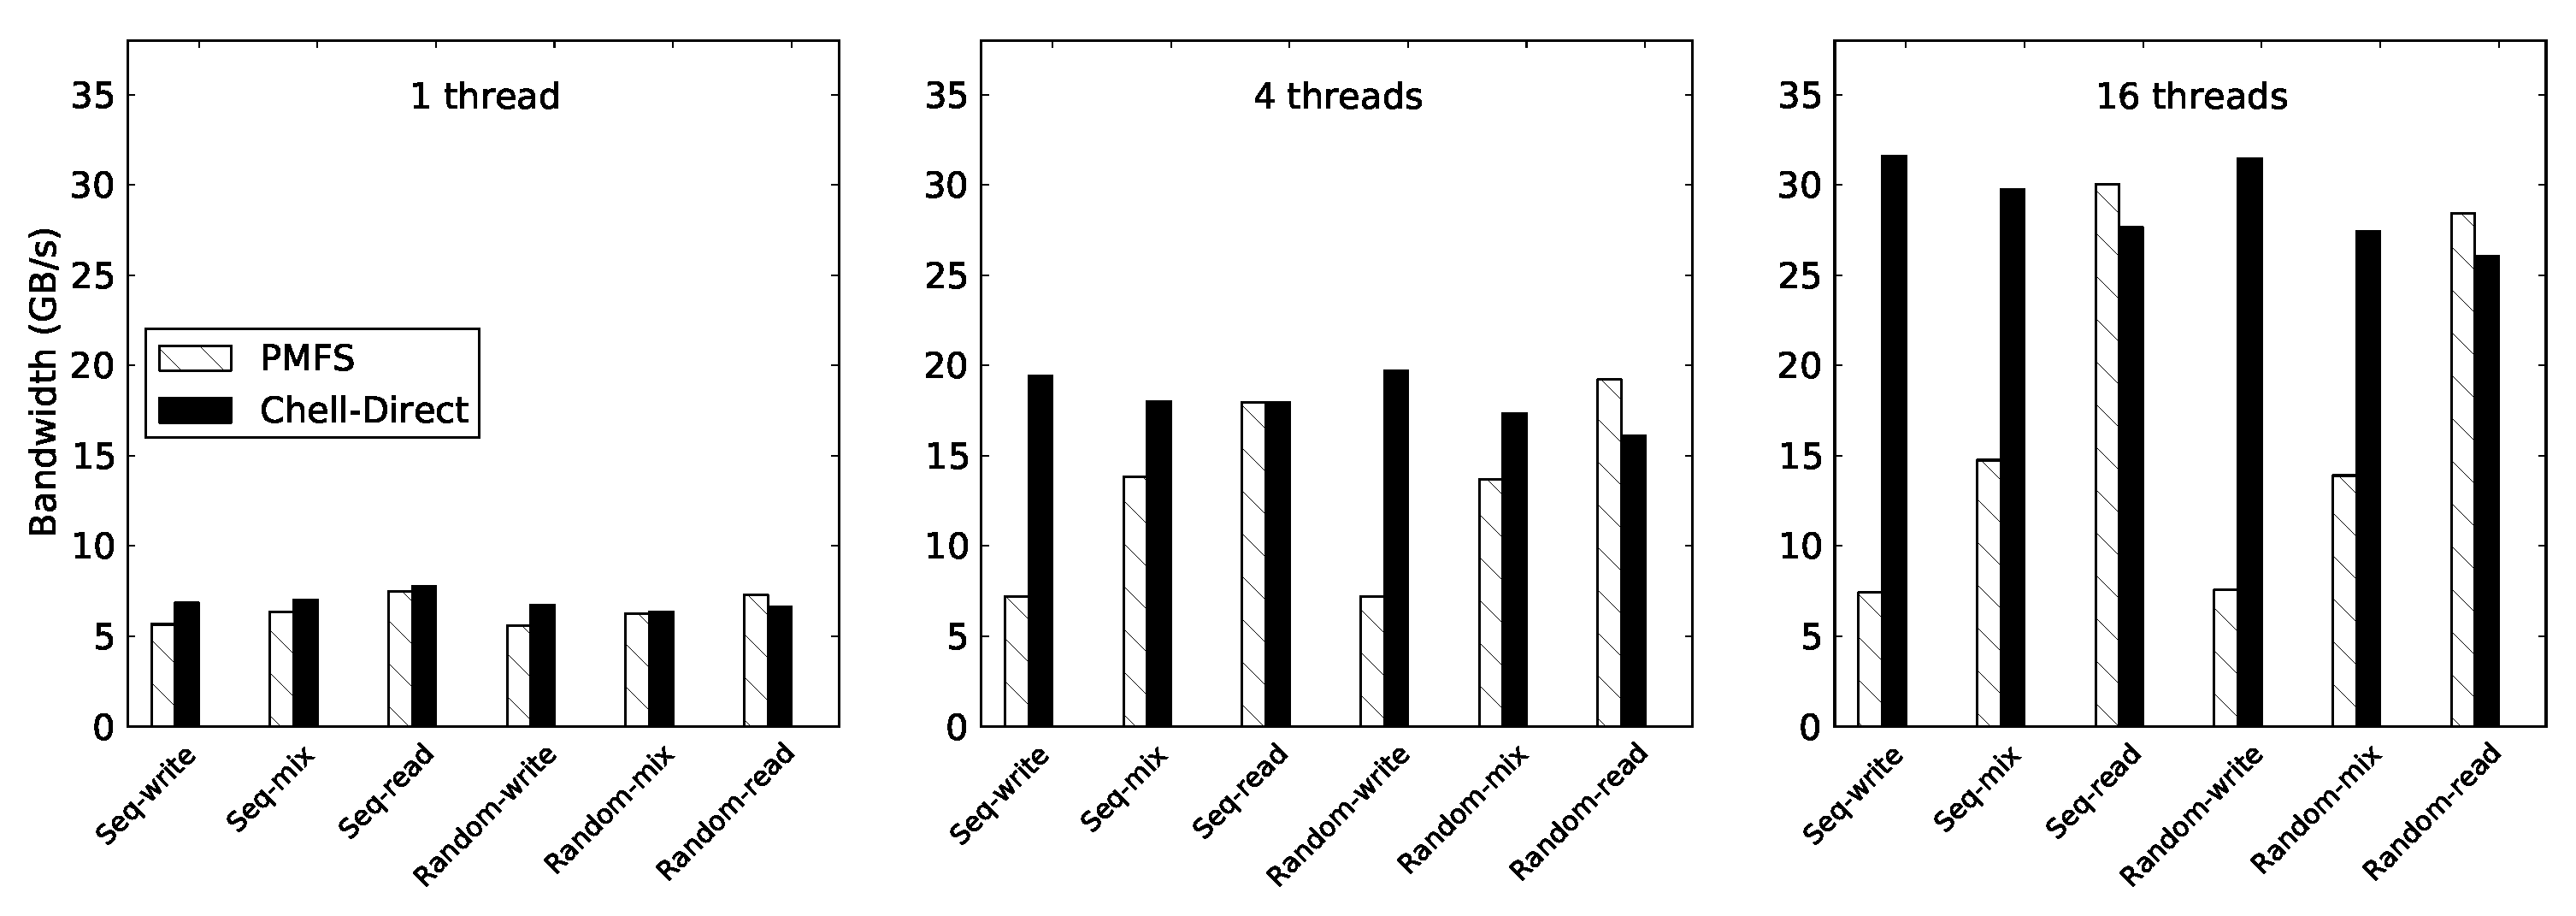
\includegraphics[width=\textwidth]{Graphs/xdd-quill.pdf}
 \vspace*{-5mm}\caption{\DAChell{} xdd bandwidth}
 \label{fig:quill-bandwidth}
\end{figure*}
}

\subsection{Macro-benchmarks}

\ignore{this section is very weak at the moment.  We need multithreaded numbers and a better description of the workload}

To measure application-level performance we ran Berkeley-DB Btree on top of
\DAChell{}. In the test, Berkeley-DB Btree application reads and writes
records to a 5.5~GB database file, and writes logs to 10~MB log files.
The workload comprises 35\% reads and 65\% writes.
The average read request size is 511 bytes, 
and average write request size is 431 bytes. The application is running with 
single thread.

\DAChell{} improves the performance by 6\% compared to PMFS.
Amdahl's law limits the gains:  NVMM is fast enough that the bottleneck is no longer in
the device I/O.  Over the test period, only about 25\% time is spent on I/O, and
\DAChell{} saves about 20\% time on I/O operations.

\begin{table}
	\centering
	\begin{tabular}{|l|c|c|}
	\hline
	\multirow{2}{*}{}&PMFS &\DAChell{}\\\hline
	&\multicolumn{2}{c|}{(Ops per second)}\\\hline
	Berkeley-DB Btree & 27160 & 29019 \\\hline
	\end{tabular}
	\vspace*{3mm}
	\caption{\figtitle{Chell-Direct Berkeley DB performance}}
	\label{table:bdb-quill}
\end{table}

\ignore{
\begin{figure}
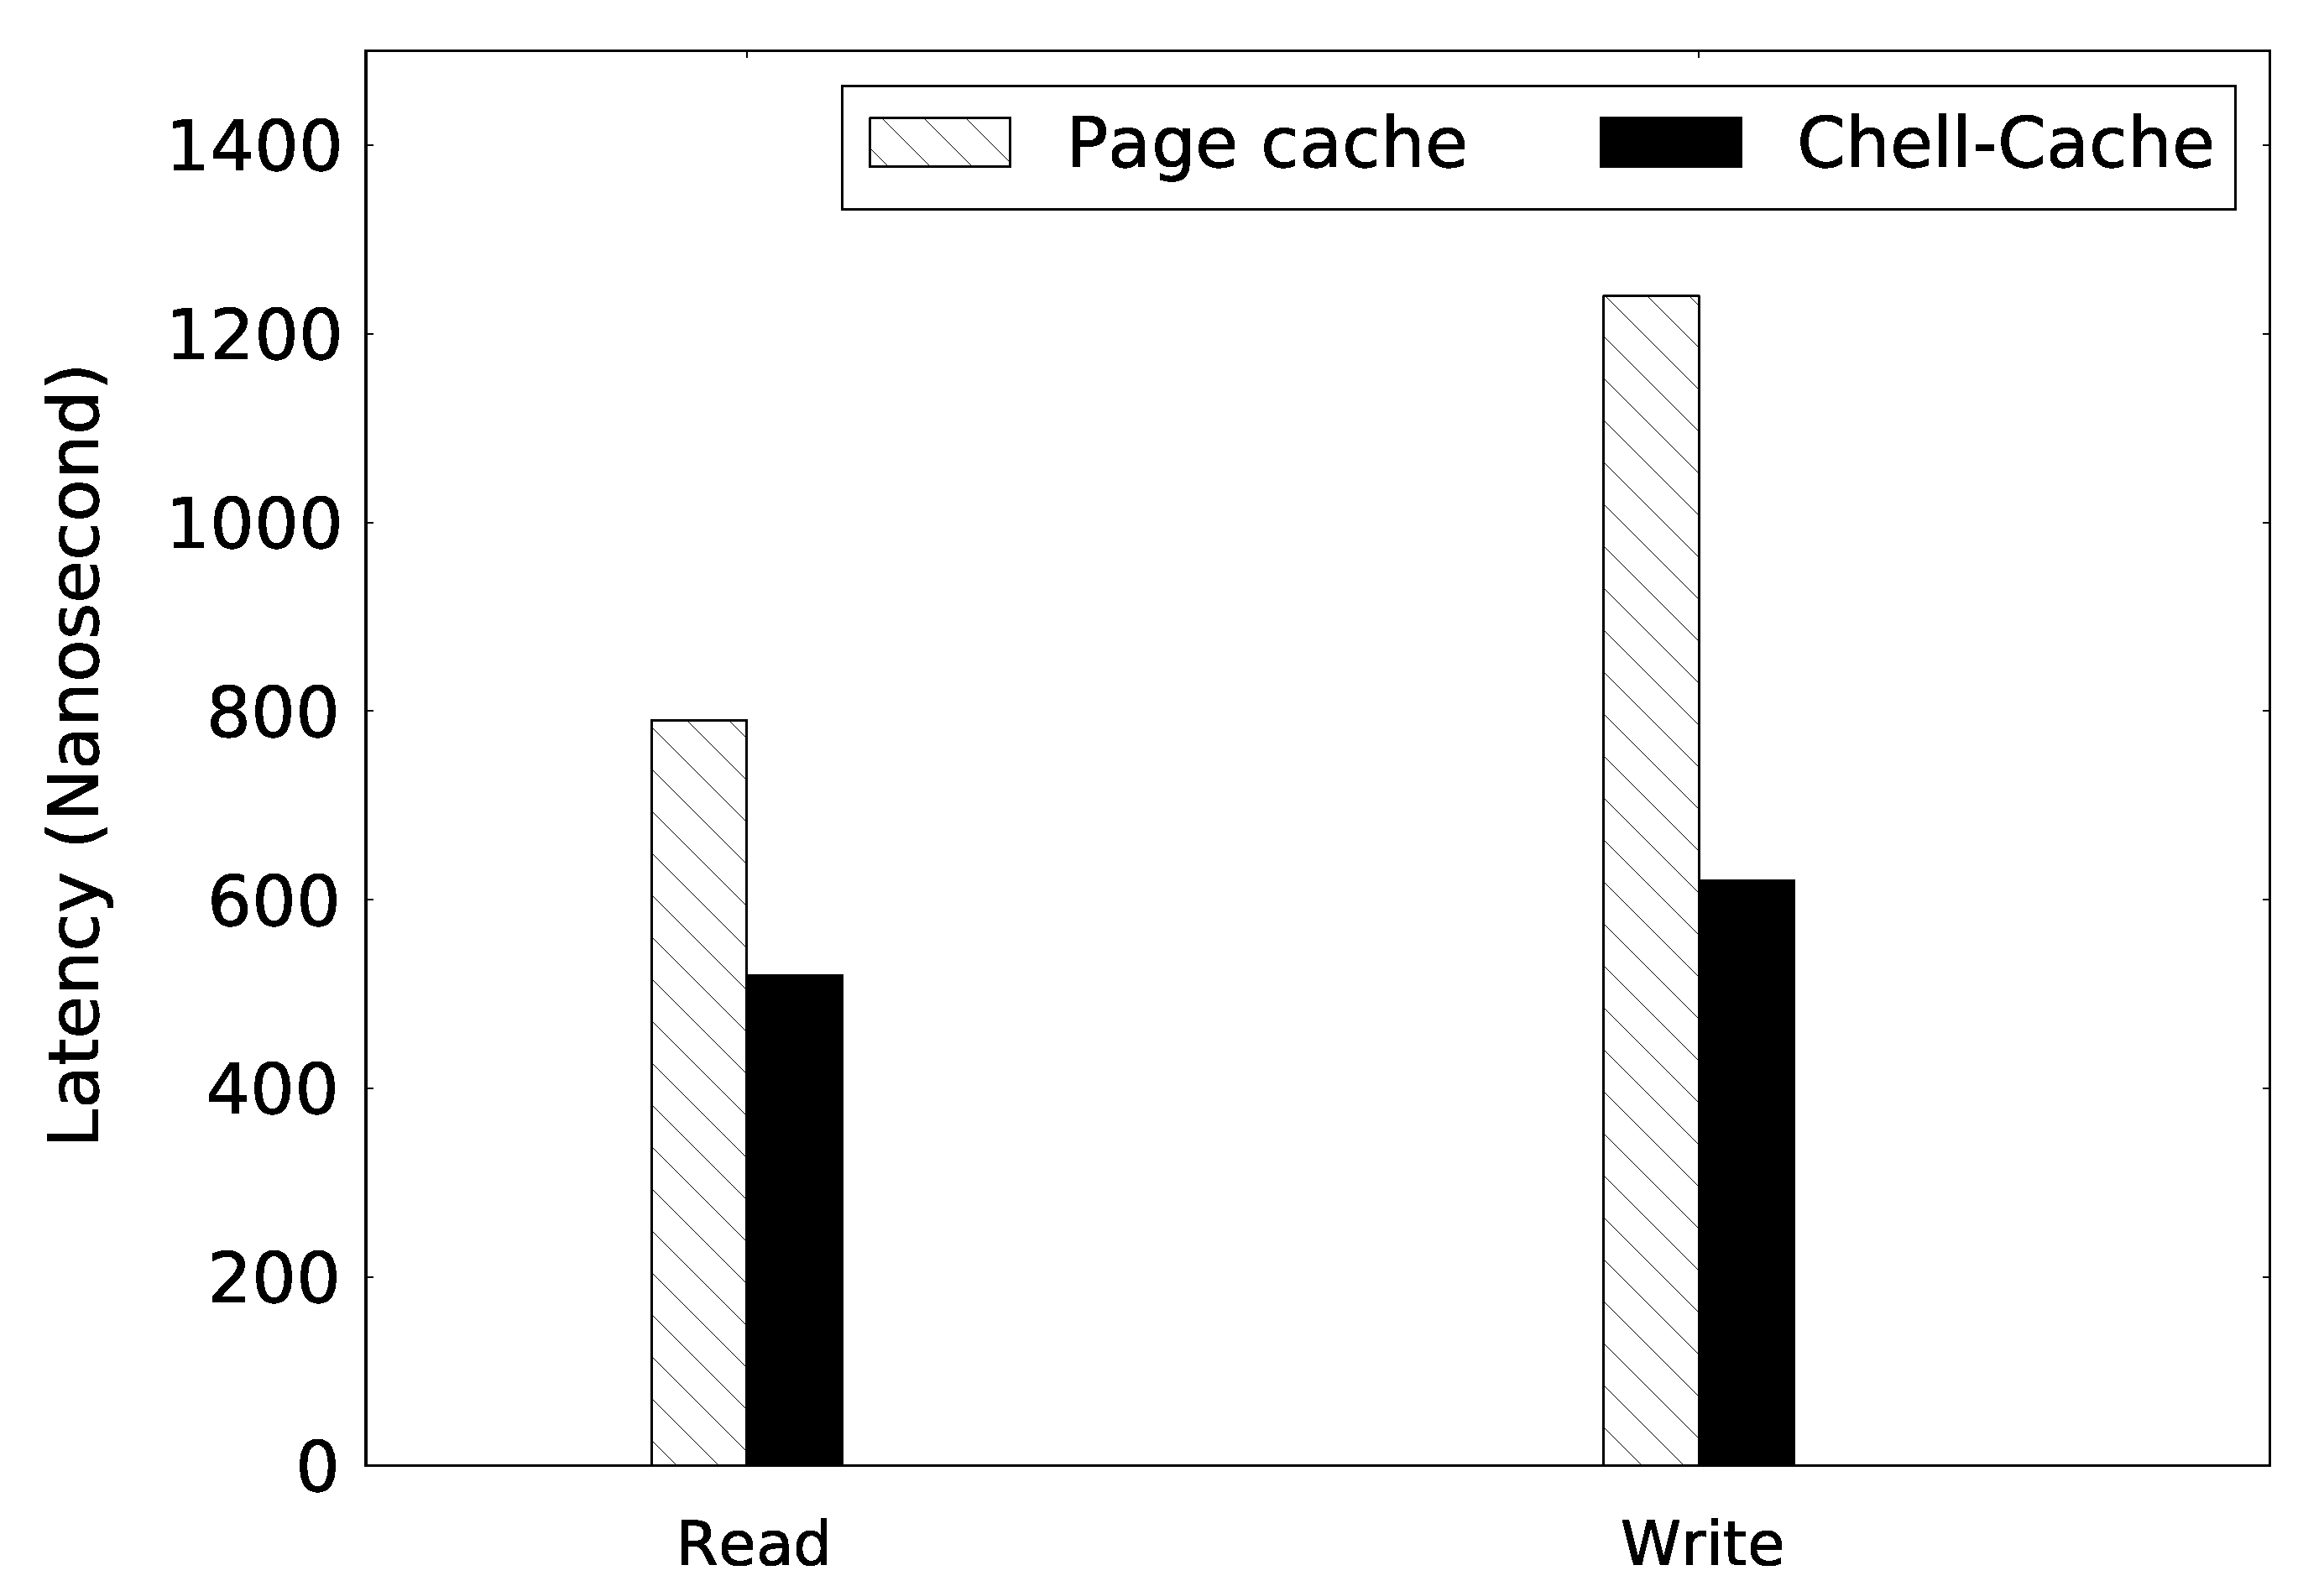
\includegraphics[width=\linewidth]{Graphs/latency.pdf}
\centering
\caption{\CChell{} 4KB access latency}
\label{fig:chell-latency}
\end{figure}
}

